\documentclass[border=10pt]{article}
\usepackage{pgfplots}
\begin{document}
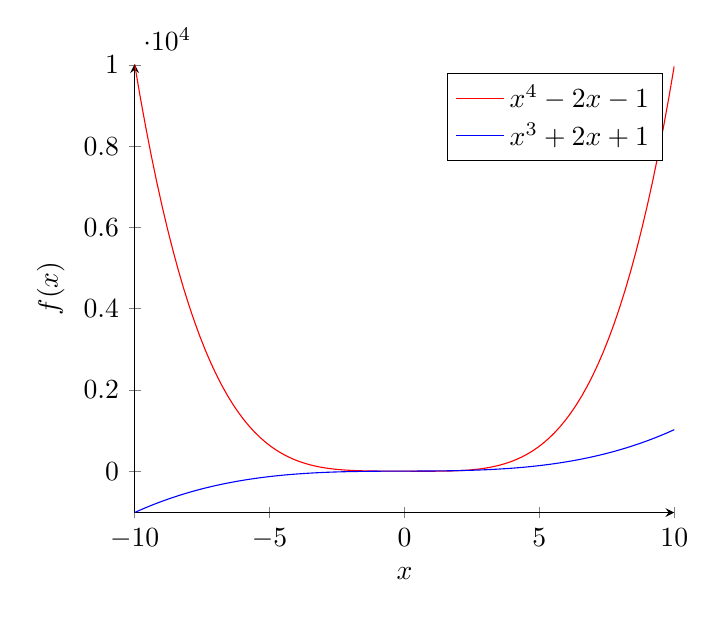
\begin{tikzpicture}
\begin{axis}[
    axis lines = left,
    xlabel = $x$,
    ylabel = {$f(x)$},
]
%Below the red parabola is defined
\addplot [
    domain=-10:10, 
    samples=100, 
    color=red,
]
{x^4 - 2*x - 1};
\addlegendentry{$x^4 - 2x - 1$}
%Here the blue parabloa is defined
\addplot [
    domain=-10:10, 
    samples=100, 
    color=blue,
    ]
    {x^3 + 2*x + 1};
\addlegendentry{$x^3 + 2x + 1$}
 
\end{axis}
\end{tikzpicture}
\end{document}

